\documentclass[8pt]{extarticle}


% -- Languages

\newif\ifen
\newif\ifde

% Use \en{Text} for english version text and \de{Text} for german version text
\newcommand{\en}[1]{\ifen#1\fi}
\newcommand{\de}[1]{\ifde#1\fi}

% Uncomment for english version
\entrue

% Uncomment for german version
%\detrue

% -- Color scheme

% Color package
\usepackage{xcolor}

% Color definitions
\definecolor{minimal-gray}{HTML}{f2f2f2}
\definecolor{minimal-black}{HTML}{131313}
\definecolor{minimal-white}{HTML}{F3F2F5}
\definecolor{minimal-red}{HTML}{C43C2D}
\definecolor{minimal-blue}{HTML}{343454}
\definecolor{minimal-yellow}{HTML}{F1C40F}
\definecolor{minimal-green}{HTML}{2D6514}
\definecolor{minimal-beige}{HTML}{D7B6A5}

% Colorbox environments
\usepackage[most]{tcolorbox}


% -- Card layout

% Layout adjustments of page (credit card format without margin)
\usepackage[paperheight=153pt, paperwidth=243pt, margin=0pt]{geometry}

% Remove paragraph indentation
\setlength{\parindent}{0pt}

% Interline spacing options
\newcommand{\largespace}{\\[2pt]}
\newcommand{\mediumspace}{\\[-3pt]}
\newcommand{\smallspace}{\\[-5pt]}

% In-box spacing around content
\newcommand{\inboxspacing}{.015\paperheight}

% Horizontal spacing of the boxes (must sum up to 1)
\newcommand{\sideboxwidth}{.425}
\newcommand{\mainboxwidth}{.575}

% Vertical spacing of the boxes (must sum up to 1)
\newcommand{\headboxheight}{.100}
\newcommand{\mainboxheight}{.880}
\newcommand{\footboxheight}{.020}

%   sideboxwidth           mainboxwidth
%  <------------> <---------------------------->
%  _____________________________________________
% |#############################################| ^
% |#######  #  # #  ## # #  #  #     # #########| |
% |####### # # # # # # # # # # # ### # #########| | headboxheight
% |####### ### # # ##  # # ### # # # #   #######| |
% |#############################################| v
% |/////////////////////                        | ^
% |/////////////////////                        | |
% |/////////////////////                        | |
% |/////////////////////                        | |
% |/////////////////////                        | | mainboxheight
% |/////////////////////                        | |
% |/////////////////////                        | |
% |/////////////////////                        | |
% |/////////////////////                        | v
% |#############################################| ^
% |#############################################| | footboxheight
% |#############################################| v


% -- Font settings

% Typesetting packages
\usepackage[letterspace=20]{microtype}
\usepackage[T1]{fontenc}

% Raleway font family
\usepackage[semibold]{raleway}
\renewcommand{\familydefault}{\sfdefault}

% Custom font commands
\newcommand{\titlefont}[1]{\uppercase{\textbf{\large{#1}}}}


% -- Additional packages

% Multirow tables
\usepackage{multirow}

% Settings for entire table columns (e.g \begin{tabular}{>{\footnotesize}rl})
\usepackage{array}

% Tikzpicture graphics
\usepackage{tikz}

% Clickable URLs
\usepackage{hyperref}
\urlstyle{same}


\begin{document}

\begin{tcbposter}[
    poster = {columns=1, rows=1, spacing=0pt},
    boxes = {sharp corners, halign=center, valign=center, boxrule=0pt}
]


% -- Headbox

\posterbox[
    colback=minimal-black,
    halign=center]
    {name=headbox,
    span=1,
    rowspan=\headboxheight}
{

    \color{white}

    \en{\titlefont{Fabio Matti | Computational Scientist}}
    \de{\titlefont{Fabio Matti | Stellenbezeichnung oder Firmenname}}
}


% -- Sidebox

\posterbox[
    colback=minimal-gray,
    valign=top,
    top=0.02\paperheight,
    halign=left,
    left=-0.01\paperwidth]
    {name=sidebar,
    below=headbox,
    column=1,
    span=\sideboxwidth,
    rowspan=\mainboxheight}
{
    \begin{tabular}{c}

       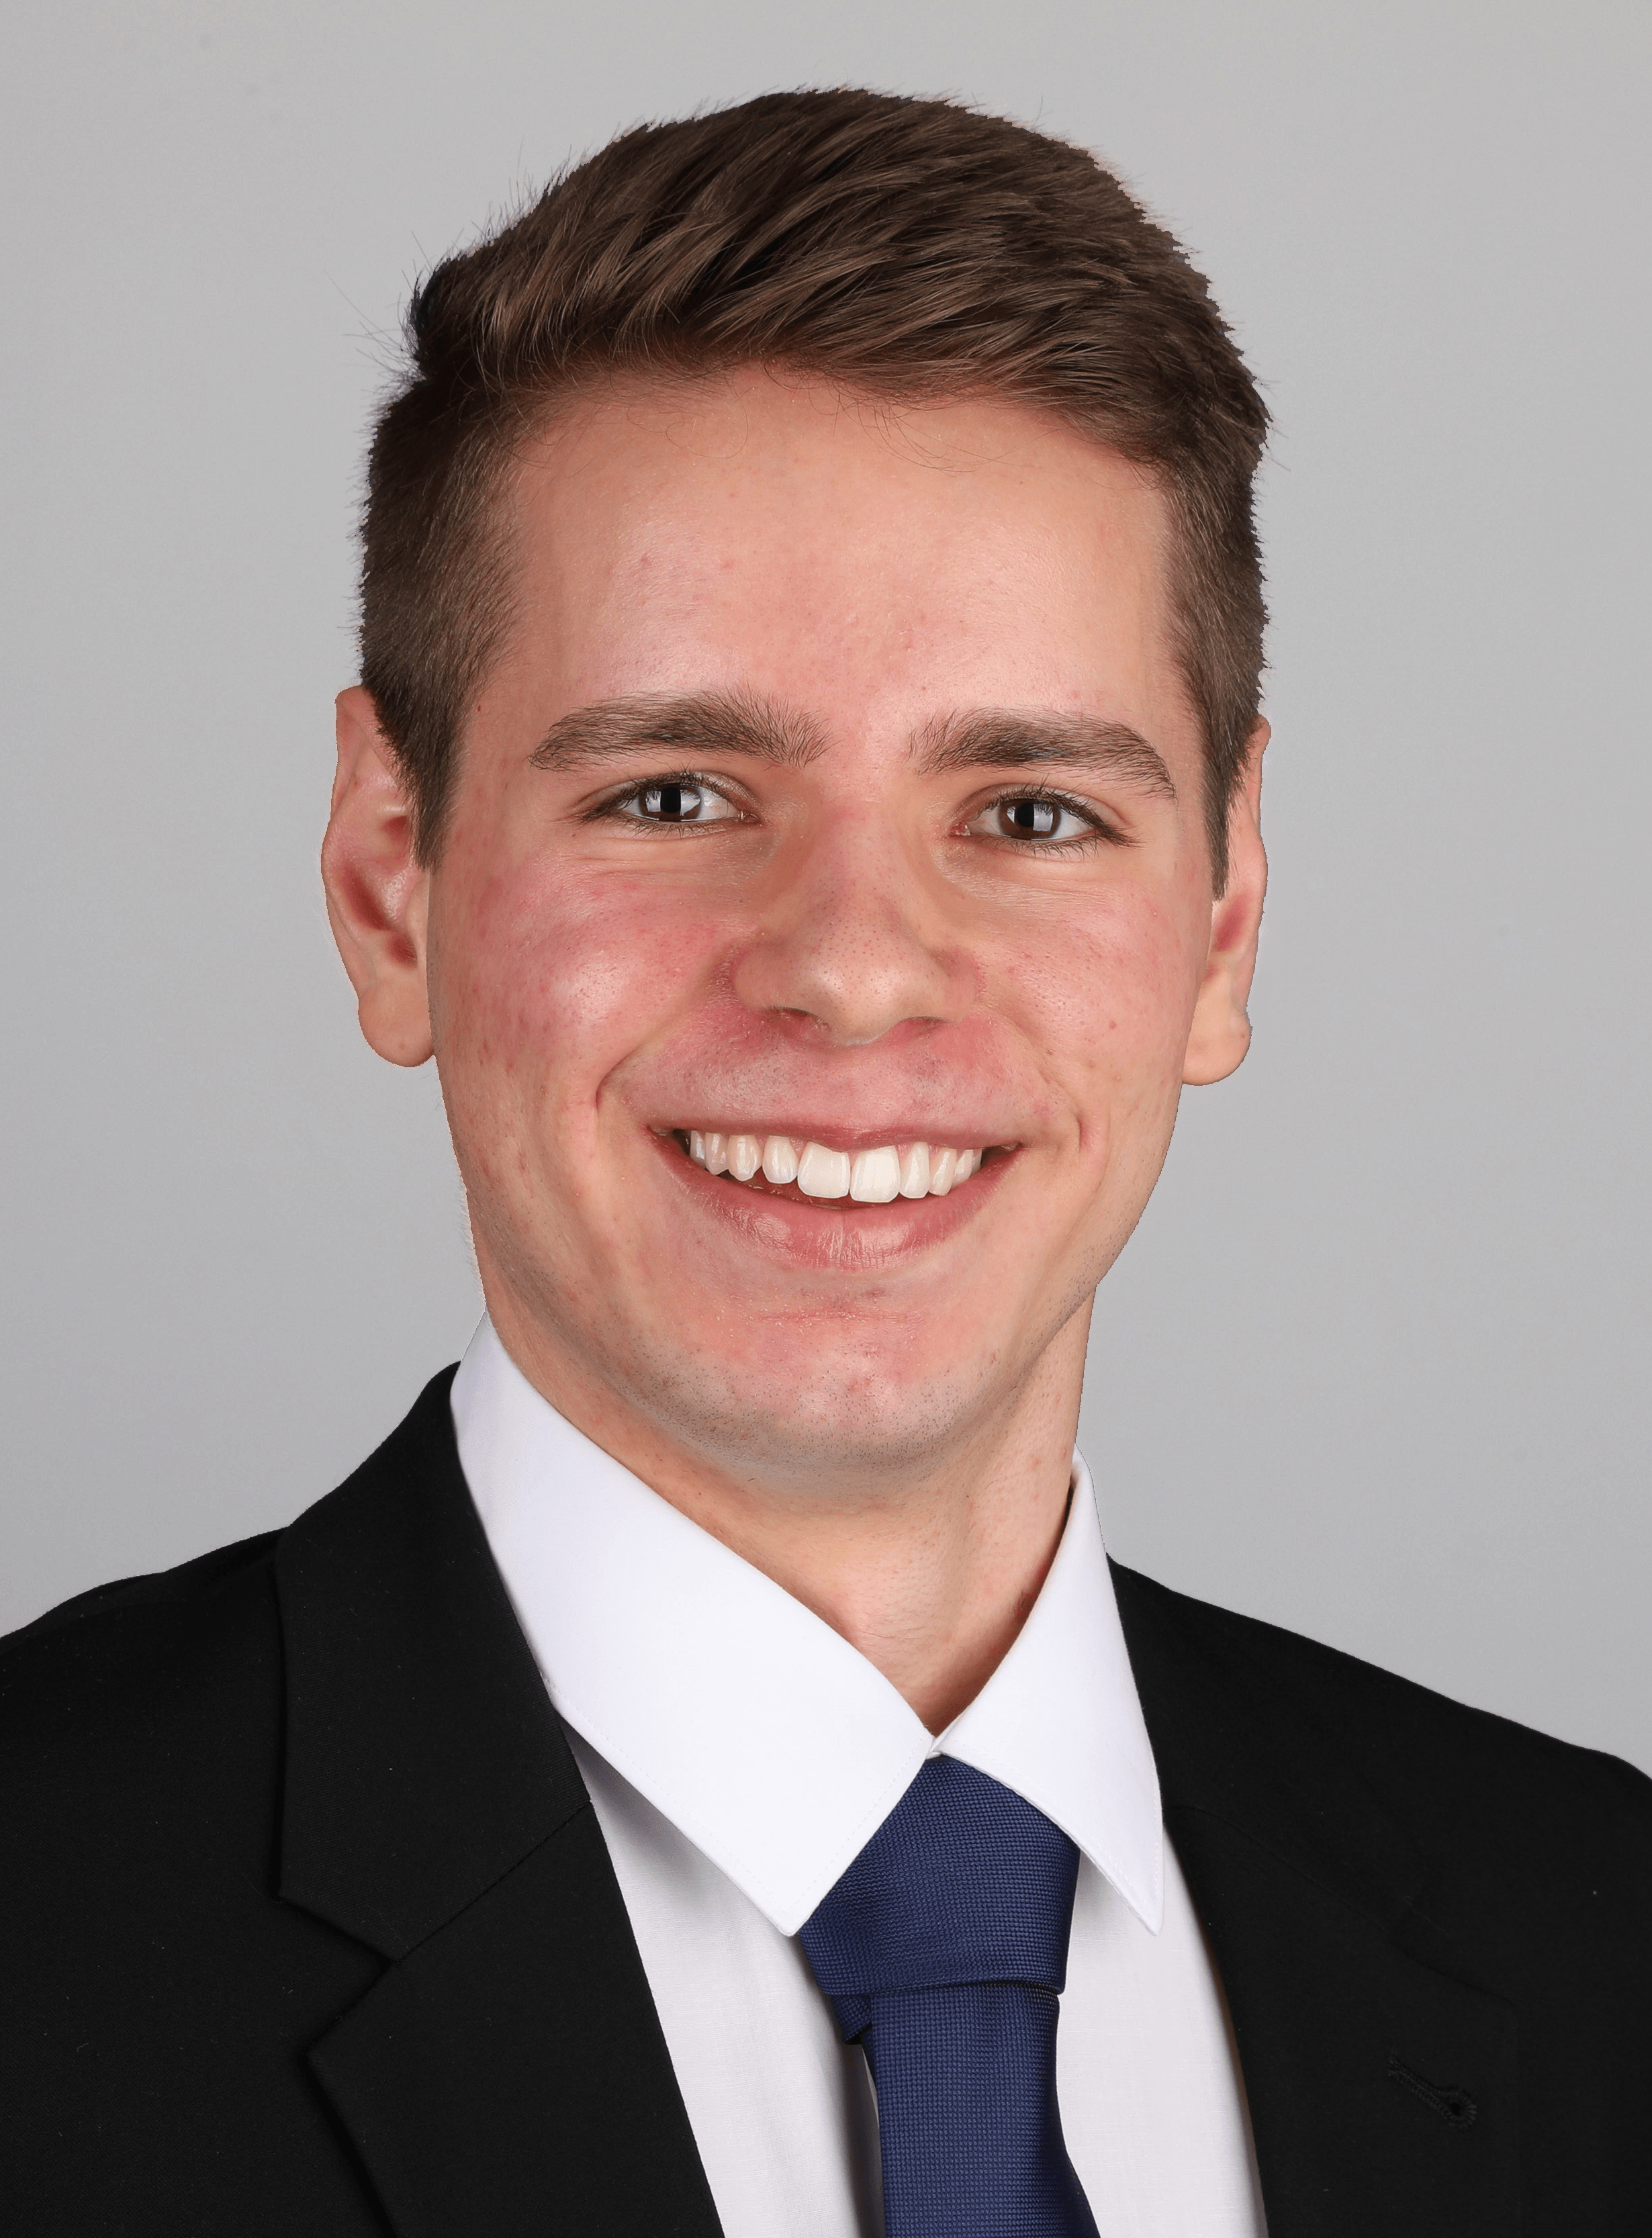
\includegraphics[scale=0.0365]{images/formal_final.png}

    \end{tabular}
}


% -- Mainbox

\posterbox[
    colback=white,
    valign=top,
    top=\inboxspacing,
    halign=left,
    left=\inboxspacing]
    {name=mainbox,
    column*=1,
    span=\mainboxwidth,
    below=headbox,
    rowspan=\mainboxheight}
{

    \color{minimal-black}

        \vspace{12pt}
    \begin{tabular}{rl}

        \multirow{2}{*}{\scalebox{0.05}{
\begin{tikzpicture}
    
    % Background
    \fill[minimal-black] (0, 0) circle (7);

    % Shell
    \fill[minimal-white] (-3.2, -5.3) rectangle (3.2, 5.3);
    \fill[minimal-black] (-2.8, -4.7) rectangle (2.8, 4.9);
    \fill[minimal-white] (-2.4, -4.3) rectangle (2.4, 4.5);

    % Button
    \fill[minimal-black] (-0.9, -5.1) rectangle (0.9, -3.9);
    \fill[minimal-white] (-0.5, -4.7) rectangle (0.5, -4.3);

\end{tikzpicture}}}
            & \textbf{\en{Phone}\de{Telefon}} \\
                & \href{tel:+41793211310}{+41 79 321 13 10} \\
                & \mediumspace

        \multirow{2}{*}{\scalebox{0.05}{
\begin{tikzpicture}

    % Background
    \fill[minimal-black] (0, 0) circle (7);
  
    % Foundation
    \fill[minimal-white] (-3.2, -5.3) rectangle (3.2, -4.7);

    % Letter
    \fill[minimal-white] (-2.8, -4.3) -- (2.8, -4.3) -- (2.8, -0.8) -- (0.0, -3.6) -- (-2.8, -0.8) -- cycle;
    \fill[minimal-white] (-2.8, -0.4) -- (0.0, -3.2) -- (2.8, -0.4) -- cycle;

    % Arrow
    \fill[minimal-white] (-0.8, 5.3) -- (-0.8, 2.4) -- (-1.8, 2.4) -- (0.0, 0.6) -- (1.8, 2.4) -- (0.8, 2.4) -- (0.8, 5.3) -- cycle;

\end{tikzpicture}}}
            & \textbf{E-Mail} \\
                & \href{mailto:fabio.matti@bluewin.ch}{fabio.matti@bluewin.ch} \\
                & \mediumspace

        \multirow{2}{*}{\scalebox{0.05}{
\begin{tikzpicture}

    % Background
    \fill[minimal-black] (0, 0) circle (7);

    % Foundation
    \fill[minimal-white] (-3.2, -5.3) rectangle (3.2, -4.7);

    % Logo
    \fill[minimal-white] (1.7, -4.3) -- (-1.7, -4.3) to[out=90, in=270] (-1.675, -4.05)
                                             to[out=190, in=330] (-3.6, -3.8)
                                             to[out=150, in=330] (-4.6, -2.35) % Tail
                                             to[out=150, in=280] (-5.0, -1.9) % Tail
                                             to[out=20, in=140] (-4.0, -2.1) % Tail
                                             to[out=320, in=160] (-3.0, -3.2) % Tail
                                             to[out=340, in=210] (-1.7, -3.1) % Tail
                                             to[out=80, in=230] (-1.25, -2.2) % Shoulder (left)
                                             to[out=180, in=230, looseness=1.15] (-3.6, 3.1) % Cheek (left)
                                             to[out=110, in=250] (-3.5, 4.9) % Ear (left)
                                             to[out=340, in=130] (-1.8, 4.1) % Ear (left)
                                             to[out=15, in=165] (1.8, 4.1) % Top
                                             to[out=50, in=200] (3.5, 4.9) % Ear (right)
                                             to[out=290, in=70] (3.6, 3.1) % Ear (right)
                                             to[out=310, in=0, looseness=1.15] (1.25, -2.2) % Cheek (right)
                                             to[out=310, in=100] (1.7, -3.1) % Shoulder (right)
                                             -- cycle;

\end{tikzpicture}}}
            & \textbf{GitHub} \\
                & \href{https://github.com/FMatti}{github.com/FMatti} \\
                & \mediumspace

        \multirow{2}{*}{\scalebox{0.05}{
\begin{tikzpicture}
    
    % Background
    \fill[minimal-black] (0, 0) circle (7);

    % i-base
    \fill[minimal-white] (-4.0, -4.0) rectangle (-2.3, 1.2);

    % i-dot
    \fill[minimal-white] (-3.15, 3.2) circle (1.0);

    % n
    \fill[minimal-white] (-1.2, -4.0) -- (-1.2, 1.2) -- (0.5, 1.2) -- (0.5, 0.5)
                 to[out=50, in=100, looseness=1.3] (4.0, -0.5)
                 -- (4.0, -4.0) -- (2.3, -4.0) -- (2.3, -0.7) 
                 to[out=100, in=80, looseness=1.1] (0.5, -0.8) -- (0.5, -4.0) -- cycle;

\end{tikzpicture}}}
            & \textbf{LinkedIn} \\
                & \href{https://linkedin.com/in/fmatti}{linkedin.com/in/FMatti} \\
                & \mediumspace

    \end{tabular}
}


% -- Footbox

\posterbox[colback=minimal-black]
           {name=blankbox2,
           below=sidebar,
           column=1,
           span=1,
           rowspan=\footboxheight}{}

\end{tcbposter}

\begin{tcbposter}[
    poster = {columns=1, rows=1, spacing=0pt},
    boxes = {sharp corners, halign=center, valign=center, boxrule=0pt}
]


% -- Headbox

\posterbox[
    colback=minimal-black,
    halign=center]
    {name=headbox,
    span=1,
    rowspan=\footboxheight}{}

    
% -- Mainbox

\posterbox[
    colback=white,
    valign=top,
    top=\inboxspacing,
    halign=left,
    left=\inboxspacing]
    {name=mainbox,
    column*=1,
    span=1,
    below=headbox,
    rowspan=\mainboxheight}
{

    \color{minimal-black}

    \begin{tabular}{>{\footnotesize}rl}

        %& \titlefont{\en{Education}\de{Bildungsweg}} \\ \hline \mediumspace

        \en{Since}\de{Seit} 09/2021
            & \en{\textbf{EPFL, Master of Science}}
            \de{\textbf{EPFL, Masterstudium}} \\
            & \en{Computational science and engineering}
            \de{Rechnergestützte Wissenschaften} \\
            & \smallspace

        09/2018 - 07/2021
            & \en{\textbf{University of Bern, Bachelor of Science}}
            \de{\textbf{Universität Bern, Bachelor of Science}} \\
            & \en{Physics with minor in mathematics}
            \de{Physik mit Minor in Mathematik} \\
            & \smallspace

       \hline \mediumspace

        07/2022 - 09/2022
            & \textbf{Prysmian Group Morges, Internship} \\
            & \en{Signal processing and machine learning}
            \de{Signal Processing und Machine Learning} \\
            & \smallspace

        \hline \mediumspace

        \en{Since}\de{Seit} 09/2022
            & \en{\textbf{EPFL, Student Assistant}}
            \de{\textbf{EPFL, Studenten Assistent}} \\
            & \en{ML (CS-433) and PCSC (MATH-458)}
            \de{ML (CS-433) und PCSC (MATH-458)} \\
            & \smallspace

        \en{Since}\de{Seit} 06/2018
            & \en{\textbf{Airbase Meiringen, NBC Staff Officer}}
            \de{\textbf{Flugplatz Meiringen, ABC Stabsoffizier}} \\
            & \en{Assistant of airbase commander}
            \de{Führungsgehile Flugplatkommandant} \\
            & \smallspace

    \end{tabular}
}



% -- Footbox

\posterbox[colback=minimal-black]
           {name=blankbox2,
           below=mainbox,
           column=1,
           span=1,
           rowspan=\headboxheight}
{      
    \color{white}

    {\scriptsize Find my full CV at \href{https://github.com/FMatti/Personal-CV}{github.com/FMatti/Personal-CV} }
}

\end{tcbposter}

\end{document}
